\section{Theorie}
\label{sec:Theorie}

Ziel des Versuches ist es die Austrittsarbeit von Elektronen aus Wolfram und eine 
Kennlinie durch thermische Emission von Elektronen zu bestimmen. \\
Durch Zufuhr von Wärme in ein Metall können Elektronen dazu gebracht werden, 
das Metall zu verlassen, dies  wird als thermische Elektronenemission 
bezeichnet. 

\subsection{Energieverteilung von Elektronen und Austrittsarbeit}

Ein Metall zeichnet sich in der Regel im kondensierter Zustand durch eine 
kristalline Gitterstruktur aus, die räumlich periodisch angeordnet ist. Die 
Elektronen sind nicht an ein Atom gebunden und bilden ein frei bewegliches 
Elektronengas. Die Potentiale innerhalb und außerhalb des Metalls werden als 
jeweils konstant genähert. Das Potential innerhalb des Metalls ist kleiner 
als außerhalb, die Differenz wird als $\varphi$ bezeichnet. Ein gutes Modell
stellt hier ein Potentialtopf mit einem symmetrischen Potential $\varphi$ dar. 
Innerhalb dieses Topfes sind die Elektronen frei verschiebbar; aus diesem Grund 
ist eine hohe Leitfähigkeit für Metalle charakteristisch. \\
Die Arbeit, die ein Elektron verrichten muss, um die Potentialschwelle zu überwinden, 
wird als Austrittsarbeit 

\begin{equation*}
W_\text{A} = e\varphi
\end{equation*}

bezeichnet. Dabei ist $e$ die Elementarladung.\\
Da Elektronen Fermionen sind, gilt für sie das Pauli-Verbot. Dieses besagt,
auf Elektronen bezogen, dass zwei von diesen in einem System nicht in allen 
Quantenzahlen übereinstimmen können. Aufgrund des Spins folgt, dass nur zwei
Elektronen dieselbe Energie haben können. Die Wahrscheinlichkeit, dass bei 
thermischen Gleichgewicht ein Zustand mit der Energie $E$ besetzt ist, wird 
durch die Fermi-Diracsche-Verteilungsfunktion

\begin{equation*}
f(E) = \frac{1}{1+\exp{\left(\frac{E-E_\text{F}}{kT}\right)}}
\end{equation*}

beschrieben, wobei $k$ die Boltzmann-Konstante und $E_\text{F}$ die Fermi-Energie 
ist, also die maximal mögliche Energie eines Elektrons bei der Temperator $T=0$.
Der qualitative VErlauf dieser Verteilungsfunktion ist in Abbildung \ref{fig:Fermi} gegeben. 

\begin{figure}
  \centering
  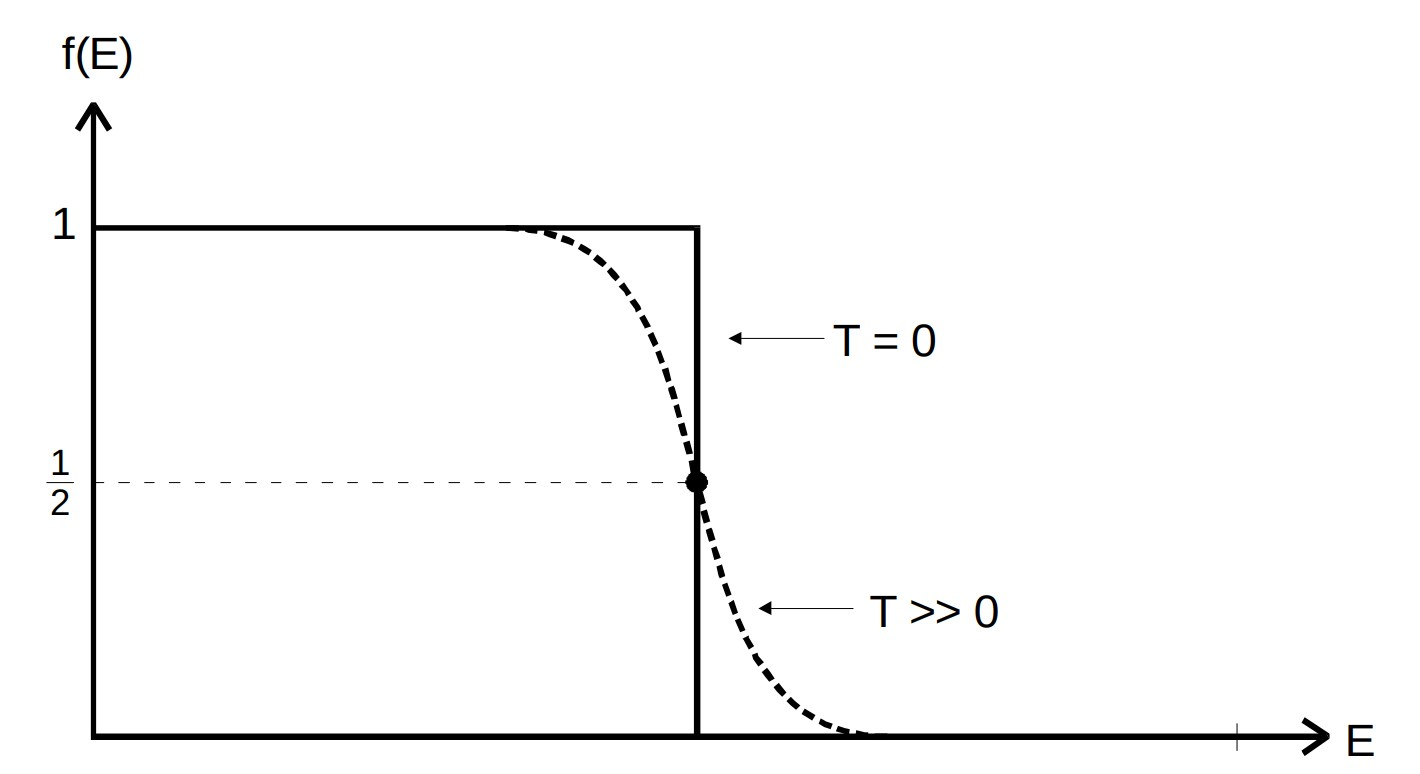
\includegraphics[scale=0.2]{content/Fermi.jpg}
  \caption{Qualitativer Verlauf der Fermi-Diracschen-Verteilungsfunktion [1].}
  \label{fig:Fermi}
\end{figure}

Bei deren Betrachtung wird deutlich, dass ein Elektron die Energiebeziehung 

\begin{equation}
E \geq E_\text{F} + e\varphi
\label{eqn:Austritt}
\end{equation}

erfüllen muss, um das Metall zu verlassen. Dieser Wert ist für die austretenden 
Elektronen selbst beim Schmelzpunkt von Wolfram noch viel größer als $kT$, daher
reicht die gute Nährung

\begin{equation}
f(E) = \exp{\left(\frac{E_\text{F}-E}{kT}\right)}.
\label{eqn:Fermi}
\end{equation}

\subsection{Sättigungsstromdichte}

Ausgehend von \eqref{eqn:Fermi} wird die Sättigungsstromdichte $j_\text{s}$ 
als die Ladung, die pro Zeit- und Fächeneinheit aus einer Metalloberfäche austreten,
in Abhängigkeit von der Temperatur definiert. Wird ein kartesisches Koordinatensystem 
verwendet, dessen $z$-Achse senkrecht auf der Metalloberfäche steht, so gilt 
für die Zahl d$\alpha$ der Elektronen in einem Impulsraum-Volumenelement $\symup{d}^3p$,
die pro Zeit- und Flächeneinheit von innen an die Grenzfläche des Metalls 
stoßen

\begin{equation*}
\symup{d}\alpha = v_\text{z} n(E) \symup{d}^3p.
\end{equation*}

Dabei ist $n(E)$ die Phasenraumdichte und $v_\text{z}$ die Geschwindigkeitskomponente
entlang der Flächennormalen. Wegen

\begin{align*}
E &= \frac{p^2}{2m}\\
&= \frac{1}{2}mv^2
\end{align*}

folgt

\begin{align*}
\symup{d}\alpha &= \frac{\partial E}{\partial p_\text{z}} n(E) \symup{d}p_\text{x} \symup{d}p_\text{y} \symup{d}p_\text{z}\\
&=n(E) \symup{d}E\symup{d}p_\text{x}\symup{d}p_\text{y},
\end{align*}

wobei $m$ die Elektronenmasse ist. Jeder Quantenzustand nimmt im sechsdimensionalen 
Phasenraum das Volumen $h$ ein, wobei $h$ das Plancksche Wirkungsquantum ist. Es 
gilt daher: 

\begin{equation*}
n(E) = \frac{2}{h³}f(E).
\end{equation*}

Der Faktor 2 kommt aus den zwei Möglichkeiten des Spins. Es gilt also 

\begin{equation*}
\symup{d}\alpha = \frac{2}{h³} \exp{\left(\frac{E_\text{F}-E}{kT}\right)}\symup{d}p\symup{d}E.
\end{equation*}

Damit die Elektronen aus dem Metall austreten können, muss \eqref{eqn:Austritt}
für $E=E_\text{kin,z}$ erfüllt sein. Das Produkt aus der Anzahl der Elektronen, 
die dieses Kirterium erfüllen, und der Elementarladung ist die Sättigungsstromdichte,
die sich zu 

\begin{equation}
j_\text{s}(T) = 4\pi\frac{emk}{h³}T^2 \exp{\left(-\frac{e\varphi}{kT}\right)}
\label{eqn:Richard}
\end{equation}

ergibt. Das Endergebnis \eqref{eqn:Richard} wird auch als Richardson-Gleichung
bezeichnet. 

\subsection{Hochvakuumdiode}

Die Messung des Sättigungsstroms wird durch eine Hochvakuumdiode realisiert. Das
gute Vakuum ist notwendig, damit die Elektronen nicht mit Luftmolekülen wechselwirken.
Die Diode erzeugt ein elektrisches Feld zwischen Anode und Glühkathode, dass die
austretenden Elektronen absaugt. An der Glühkathode liegt eine Heizspannung an, die
einen Strom durch den Wolframdraht fließen lässt, der das Wolfram auf $\SI{1000}{\kelvin}$
bis $\SI{3000}{\kelvin}$ erhitzt. Die Emission der Anode ist deutlich geringer
als die der Kathode. 

\subsection{Die Langmuir-Schottkysche Raumladungsgleichung}

Bei gegebener Kathodentemperatur ist der Anodenstrom von der Anodenspannung 
abhängig. Ist die Spannung zu niedrig, so erreichen nicht alle Elektronen
die Anoden. Dies geschieht erst bei hinreichend hoher Anodenspannung. Dann ist 
der Strom von der Spannung unabhängig. \\
Eine Diode verletzt das Ohmesche Gesetz, da die Elektronen eine Beschleunigung 
in Richtung der Anode erfahren, insbesondere tritt eine Inhomogenität der 
Ladungsdichte auf. Die Raumladungsdichte nimmt zur Anode hin ab, da sich im 
Bereich der Glühkathode die meisten Elektronen befinden. Auf Grund der 
Kontinutitätsbedingung ist die Stromdichte an jeder Stelle konstant. Wegen

\begin{equation}
j = \rho v
\label{eqn:dichte}
\end{equation}

folgt, dass für kleine Geschwindigkeiten $v$ der Elektronen die Raumladungsdichte
$\rho$ groß sein muss, dies ist aber vor allem im Bereich der Glühkathode der Fall.
Sie ist so groß, dass die das Feld der angelegten Spannung abschirmt. Daraus 
folgt also, dass der Diodenstrom kleiner als der erwartete Sättigungsstrom 
\eqref{eqn:Richard} ist. \\
Für den quantitativen Zusammenhang wird von der Poisson-Gleichung 

\begin{equation}
\frac{\symup{d}²U}{\symup{d}x²} = \frac{\rho(x)}{\epsilon_0},
\label{eqn:Poisson}
\end{equation}

wobei $U$ das elektrische Potential und $\epsilon_0$ die elektrische 
Feldkonstante ist, ausgegangen unter den einfachen Annahme, dass Anode und
Kathode Oberflächen unendlicher Ausdehnung mit dem Abstand $a$ sind. Damit 
hängen $v$ und $\rho$ nur von der Ortskoordinate $x$ ab. Mit Hilfe von 
\eqref{eqn:dichte} und der Äquivalenz von elektrischer und kinetischer 
Energie lässt sich \eqref{ewn:Poisson} integrieren. Dabei ergibt sich 
für das Potential 

\begin{equation*}
U(x) = \left(s\sqrt{\frac{j}{4\epsilon_0\sqrt{\frac{2e}{m}}}}x\right)^{\frac{4}{3}}.
\end{equation*}

Außerdem gilt für das elektrische Feld und die Ladungsdichte 

\begin{align*}
E(x) &\propto x^{\frac{1}{3}},\\
\rho(x) &\propto x^{-\frac{2}{3}}.
\end{align*}

Für die Stromdichte gilt schließlich 

\begin{equation}
j = \frac{4}{9}\epsilon_0 \sqrt{\frac{2e}{m}} \frac{1}{a²} U^{\frac{3}{2}}.
\label{eqn:Langmuir}
\end{equation}

Dieses Gesetz, das die korrekte Proportionalität zwischen Stromdichte und 
Potential angibt, wird das Langmuir-Schottkysche Raumladungsgesetz genannt. 
Der Gültigkeitsbereich von \eqref{eqn:Langmuir} im $j-U$-Diagramm einer 
Hochvakuumdiode nennt man das Raumladungsgebiet. 

\subsection{Anlaufstromgebiet einer Hochvakuumdiode}

Nach \eqref{eqn:Langmuir} sollte fpür $U=0$ die Stromdichte verschwinden, 
experimentell ergibt sich jedoch ein geringer Anodenstrom. Für $T > 0$ gibt 
es laut \eqref{eqn:Fermi} endlich viele Elektronen, deren Energie größer
als die Austrittsarbeit ist. Dadurch erhalten die Elektronen eine Restenergie

\begin{equation*}
\symup{\Delta} E = E-(E_\text{F}+e\varphi),
\end{equation*}

sodass sie gegen ein Feld anlaufen können. Die Menge dieser Elektronen wird
daher als Anlaufstrom bezeichnet. Das Anodenmaterial besitzt meistens eine höhere
Austrittsarbeit als die Kathode. Durch die externe leitende Verbindung werden 
die Fermi-Oberflächen $E=E_\text{F}$ auf das selbe Niveau gebracht. Bei einem 
Potential $U$ entsteht eine Potentialdifferenz von $eU$. Um die Anode zu erreichen,
muss $E \geq e\varphi_\text{A}+eU$ sein, wobei $e\varphi_\text{A}$ die Austrittsarbeit
der Anode ist. Die Zahl der Leitungselektronen zwischen $E$ und $E+\symup{d}E$ hängt
exponentiell von $E$ ab, somit hängt auch die Anlaufstromstärke vom äußeren 
Potential ab: 

\begin{equation*}
j(U) = j_0 \exp{\left(-\frac{e\varphi_\text{A}+eU}{kT}\right)}\propto \exp{\left(-\frac{eU}{kT}\right)}.
\label{eqn:exponent}
\end{equation*}

\subsection{Kennlinie einer Hochvakuumdiode}

Als Kennlinie wird der Zusammenhang zwischen Anodenstrom $I$ und der von außen
angelegten Spannung $U$ definiert. Wie in Abbildung \ref{fig:Kennlinie} gliedert sich die 
Kennlinie in die Bereiche Anlaufstrom-, Raumladungs-, und Sättigungsstromgebiet.
Im ersten Bereich gibt es einen exponentiellen Zusammenhang zwischen $I$ und $U$.
Im anschließenden Raumladungsgebiet gibt es eine $\sqrt{U³}$-Abhängigkeit. 
Gleichung \eqref{eqn:Langmuir} kann nicht für beliebig hohe Spannungen gültig 
sein, da die Zahl der pro Zeiteinheit emittierten Elektronen gemäß \eqref{eqn:Richard}
nur von der Temperatur, aber nicht von der Anodenspannung abhängt. Der Strom strebt 
einem Sättigungsstrom $I_\text{S}$ zu, was den kontinuierlichen Übergang in
das Sättigungsstromgebiet kennzeichnet. 

\begin{figure}
  \centering
  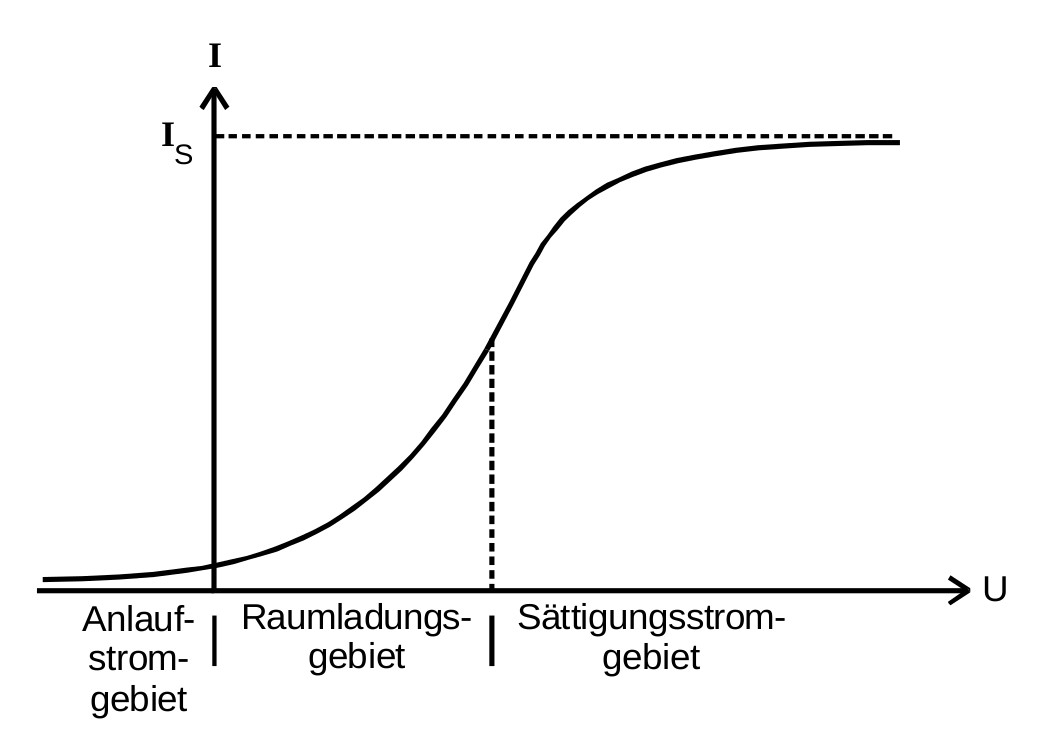
\includegraphics[scale=0.2]{content/Kennlinie.jpg}
  \caption{Beispiel einer Kennlinie [1].}
  \label{fig:Kennlinie}
\end{figure}

\cite{sample}
